\documentclass[tikz,border=10pt]{standalone}
\begin{document}
% scale: 0.021333 cm per px, centre (224.2,222), y flipped
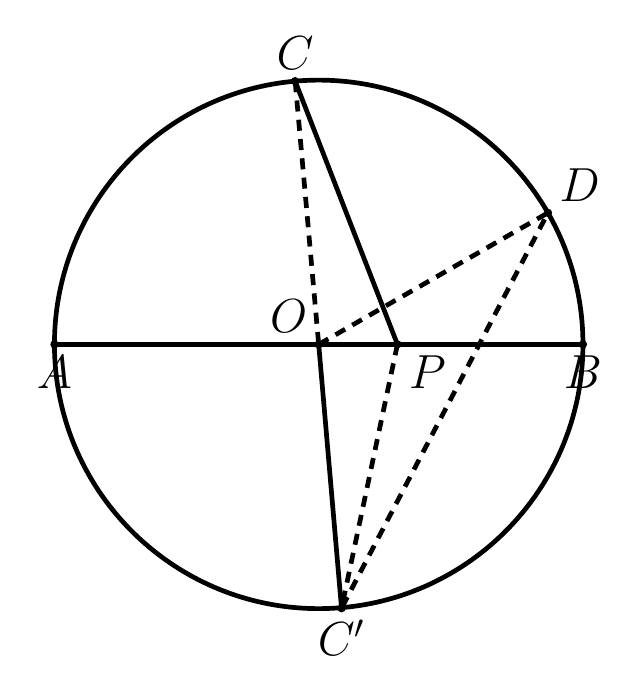
\begin{tikzpicture}[line join=round, line width=1.7pt,
    lbl/.style={font=\fontsize{18}{21.6}\selectfont},
    dashd/.style={dash pattern=on 4pt off 3pt}]

% named coordinates (cm)
\coordinate (O)  at (0,0);
\coordinate (A)  at (-3.356,0);
\coordinate (B)  at (3.356,0);
\coordinate (P)  at (1.000,0);
\coordinate (C)  at (-0.299,3.343);
\coordinate (Cp) at (0.290,-3.351);
\coordinate (D)  at (2.912,1.671);

% circle of radius 157.3 px
\draw (O) circle (3.356);

% solid: diameter AB, C-P, O-C'
\draw (A) -- (B);
\draw (C) -- (P);
\draw (O) -- (Cp);

% dashed (proper dash pattern): C-O, O-D, P-C', D-C'
\draw[dashd] (C) -- (O);
\draw[dashd] (O) -- (D);
\draw[dashd] (P) -- (Cp) -- (D);

% small filled vertex dots at O, A, B, C, D, C', P
\fill (O)  circle (1.5pt);
\fill (A)  circle (1.5pt);
\fill (B)  circle (1.5pt);
\fill (C)  circle (1.5pt);
\fill (D)  circle (1.5pt);
\fill (Cp) circle (1.5pt);
\fill (P)  circle (1.5pt);

% labels
\node[below, lbl] at (A) {$A$};
\node[below, lbl] at (B) {$B$};
\node[above left, lbl] at (O) {$O$};
\node[below right, lbl] at (P) {$P$};
\node[above, lbl] at (C) {$C$};
\node[below, lbl] at (Cp) {$C'$};
\node[above right, lbl] at (D) {$D$};

\end{tikzpicture}
\end{document}